\documentclass[a4paper]{article}
\usepackage[utf8]{inputenc}
\usepackage{geometry}
\usepackage{graphicx}

\usepackage[T1]{fontenc}
\usepackage{lmodern}
\usepackage[ngerman]{babel}

\usepackage{float}

%\geometry{a4paper, left=2cm, right=2cm, top=2cm, bottom=2cm}
\title{Ein Testdokument}
\author{Otto Normalverbraucher}
\date{05. Januar 2004}

\begin{document}


\maketitle

\newpage

\tableofcontents

\newpage


\section{Einleitung}

\section{Konzept}

Die Idee ist, dass Serien-Interessierte über ihre zuvor favorisierten Serien und abonnierten Interessen benachrichtigt werden, sobald eine Episode dieser Serie im TV ausgestrahlt wird.

Der Serien-Interessierte soll Zugriff auf einen Pool von Serien bekommen, die auf einem Server gespeichert und verwaltet werden.
Die einzelnen Serien soll der Nutzer dann favorisieren/abonnieren können um dann über die TV-Ausstrahlung informiert zu werden.
Außerdem soll die Möglichkeit bestehen eine Episode zu bewerten und als gesehen/ungesehen zu markieren. Es besteht zudem die Möglichkeiten Serien in Listen einzuordnen und zu verwalten. (definitiv automatische Watchlist/Seenlist)

Die Server-Anwendung soll die Nutzer über die TV-Austrahlung einer Episode einer zuvor favorisierten Serie in einem vom Benutzer definierten Zeitraum informiert werden. Jeder Eintrag einer Serie enthalt zudem Informationen wie Genre, anhand derer Abonnentenl bezüglich eines bestimmten Themas, zusätzliche Benachrichtigungen empfangen.

Ein **Content-Admin** soll erweiterte Rechte bekommen, um die Content-Verwaltung zu übernehmen. Die Anwendung soll das Anlegen, Bearbeiten und Löschen von Serien bzw Episoden ermöglichen. Zudem ist somit das Korrigieren von Fehlern möglich, die von Usern eingeschickt werden.

\subsection{Zusatz - Freunde}
Serien-Interessierte sollen sich gegenseitig hinzufügen/abonnieren können um sich gegenseitig zu benachrichtigen, zum Beispiel in Form von Freund X schaut gerade Y, Freund Z hat Serie/Episode mit 8,0 bewertet oder Freund Y empfiehlt Dir Serie W.


\subsection{Umsetzung}
Die Anwendung ermöglicht den Austausch von Informationen zwischen Server und Anwender entsprechend den jeweiligen Funktionen.

\subsubsection{Synchrone Datenübertragung}

Zum einen hat der Anwender direkt die Möglichkeit auf Informationen in Form von Daten zuzugreifen und diese zu Manipulieren.

\begin{itemize}
\item
Serien-Interessierte
	\begin{itemize}
	\item
    Markieren von Episoden
    	\begin{itemize}
    	\item
     	Gesehen/Nicht gesehen
     	\end{itemize}
    \item
    Bewertung einer Episode
      	\begin{itemize}
      	\item
        Kommentar
        \item
        Bewertung in Zahlen
        \end{itemize}
     \item
     Fehlermeldung
     	\begin{itemize}
     	\item
        geänderte Sendezeit, fehlerhaftes Datum
        \end{itemize}
     \item
     Listen
     	\begin{itemize}
     	\item
    	Ausgabe (Un)Watched
    	\item
     	Ausgabe vorhandene Serien
     	\item
     	Ausgabe Follower/Following (?)
     	\end{itemize}
     \item
     Favorisierung
   	  	\begin{itemize}
   	  	\item
   	  	Anlegen
   	  	\item
   	  	Löschen
   	  	\item
   	  	Bearbeiten
   	  		\begin{itemize}
   	  		\item
   	  	    Zeitpunkt der Benachrichtigung
   	  	    \end{itemize}
		\end{itemize}
	\end{itemize}
	\item
	Content-Admin
		\begin{itemize}
		\item
		Verwaltung der Episoden
			\begin{itemize}
			\item
			Anlegen
			\item
			Löschen
			\item
			Bearbeiten
			\end{itemize}
		\end{itemize}
\end{itemize}


\subsubsection{Asynchrone Datenübertragung}

Ein weiterer Aspekt ist das Anfordern von Informationen, wobei die entsprechenden Informationen von Seiten des Servers von Bedingungen abhängig gesendet werden, was auch mehrfach geschehen kann.

\begin{itemize}
\item
Serien-Interessierte
	\begin{itemize}
	\item
    Benachrichtung bei TV-Austrahlung
    \item
    Freunde mit gleicher Favorisierung bei Serienstart mit Check-in benachrichtigen (?)
	    \begin{itemize}
	    \item
         Freund X schaut auch W
         \end{itemize}
    Empfehlung einer Serie von Freund(e) anzeigen (?)
    \end{itemize}
\item
Content-Admin
	\begin{itemize}
	\item
    Benachrichtung bei Fehlermeldung durch User
    \end{itemize}
\end{itemize}



\begin{figure}[H]
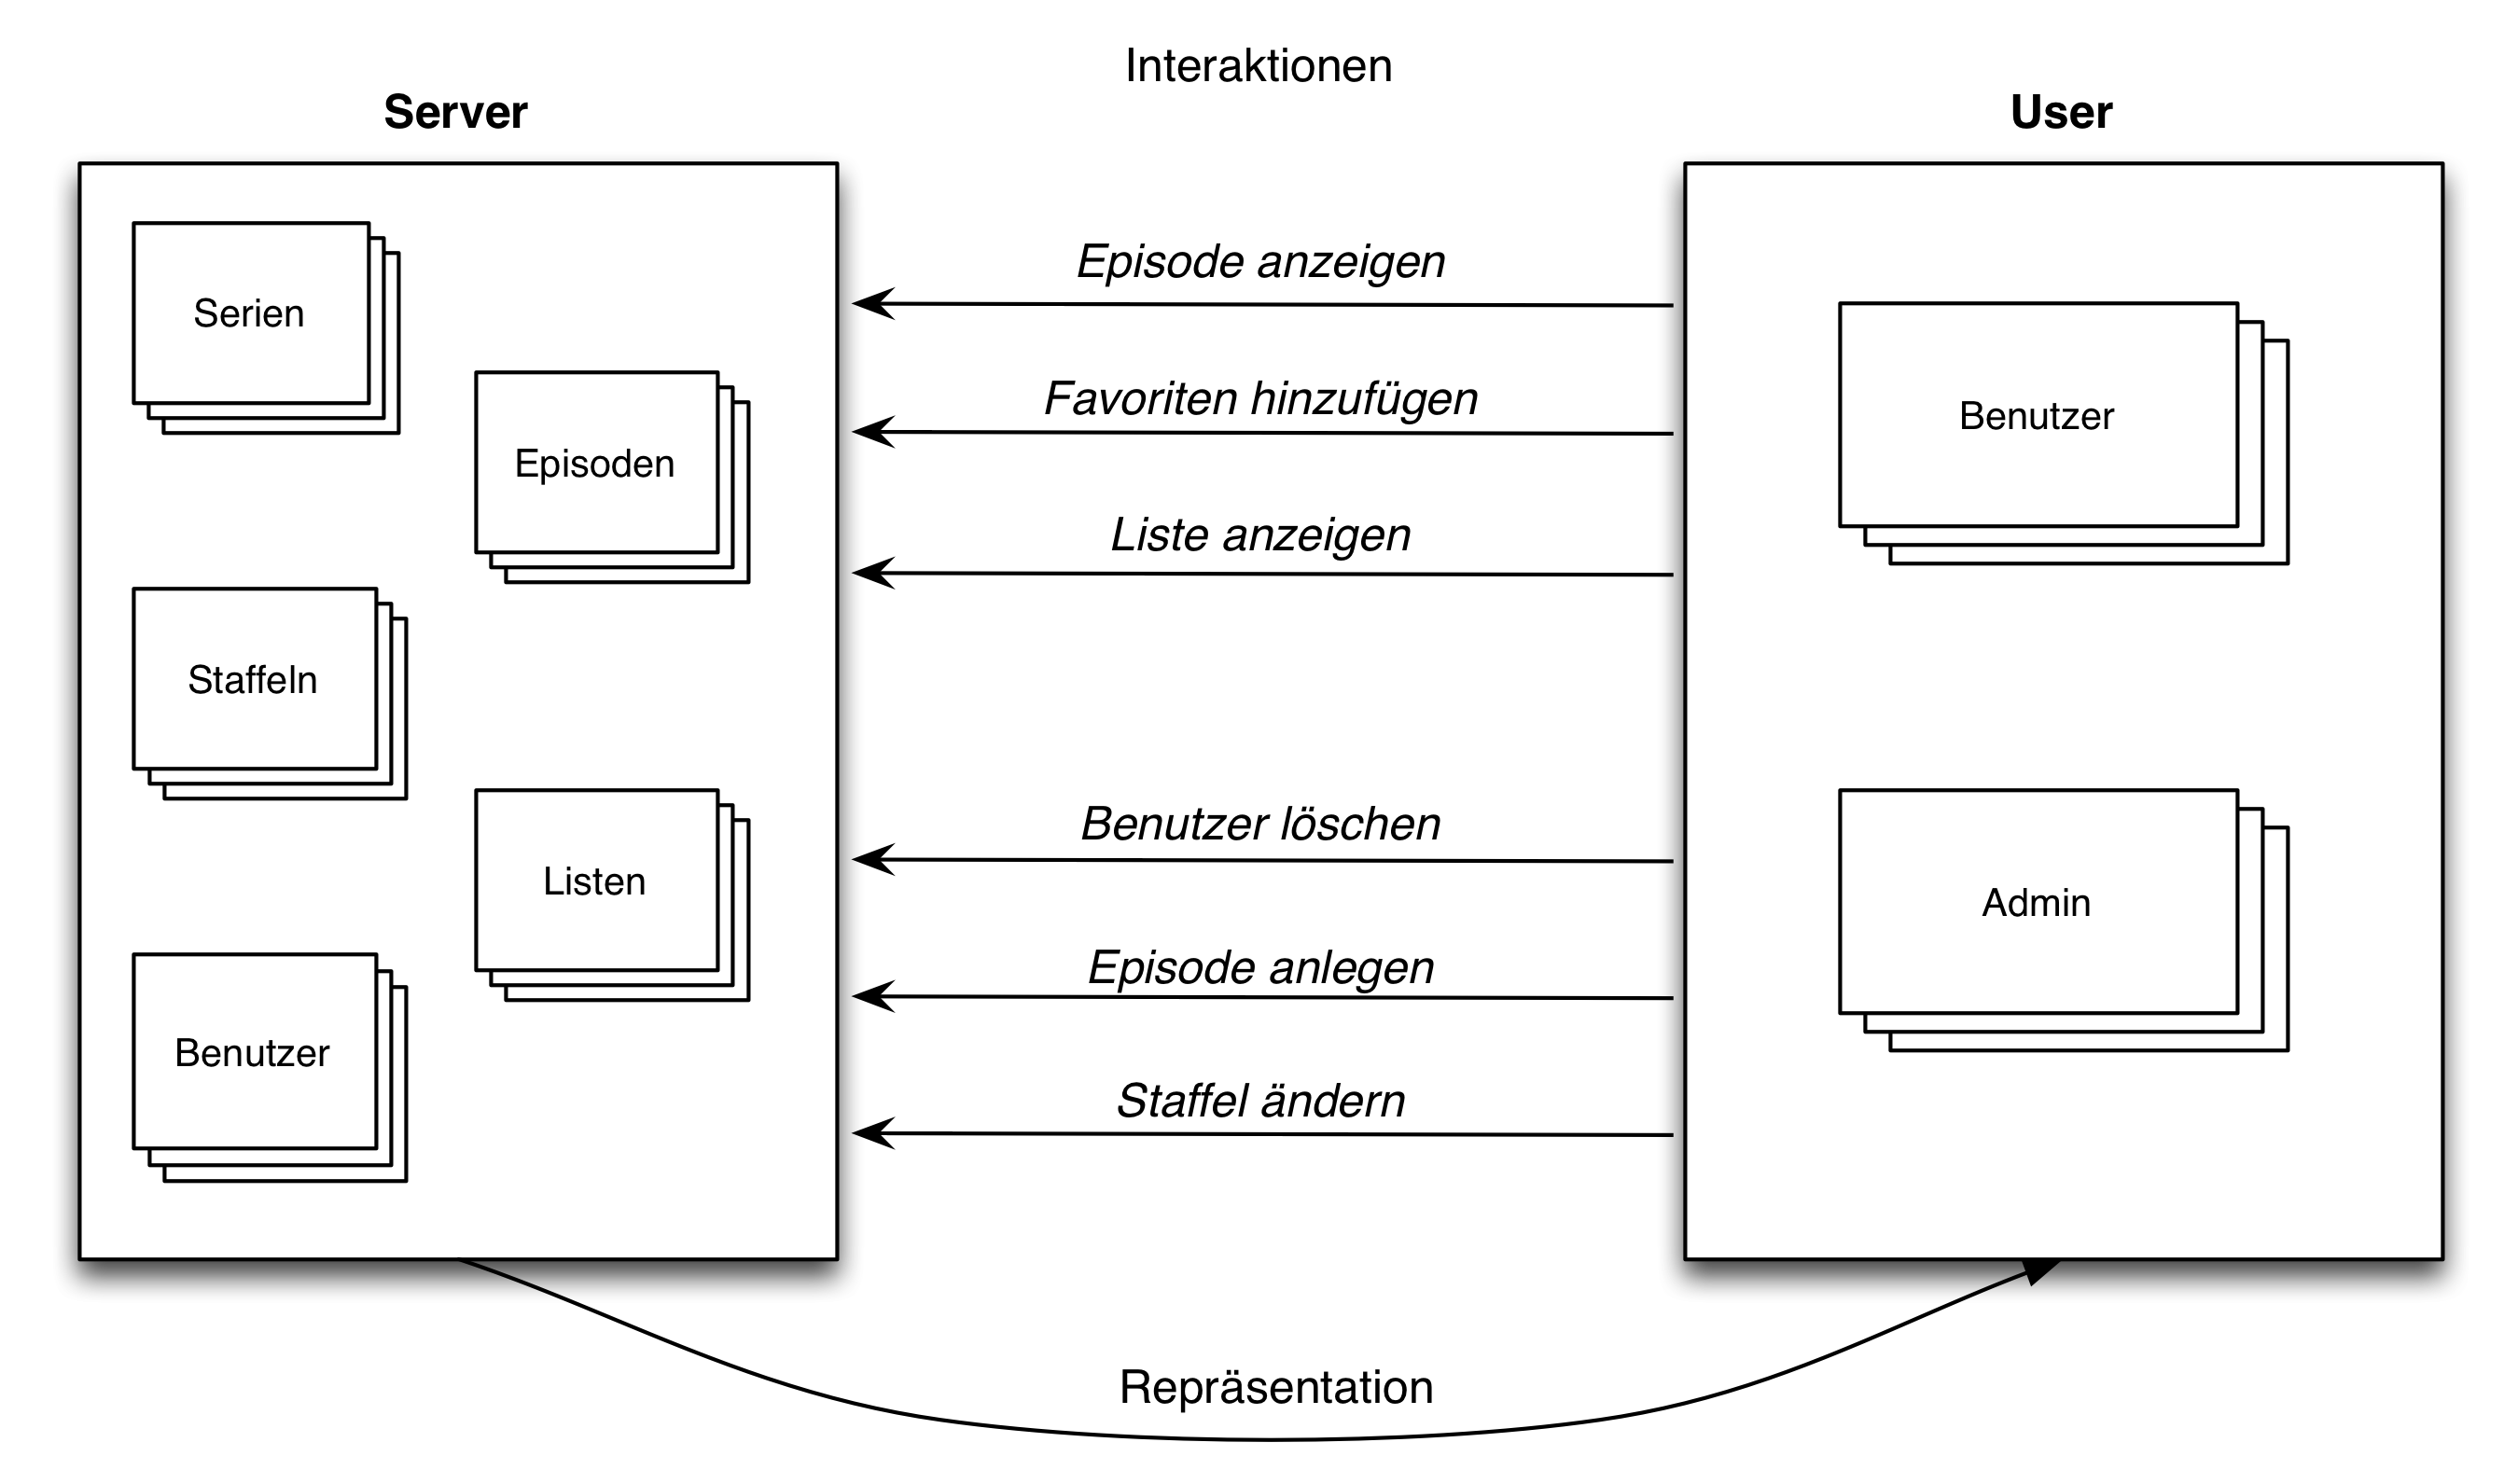
\includegraphics[width=1\textwidth]{images/kommunikationsablaeufe.png}
\caption{Synchrone Kommunikationsabläufe}
\label{kommunikationsablaeufe}
\end{figure}


\begin{figure}[H]
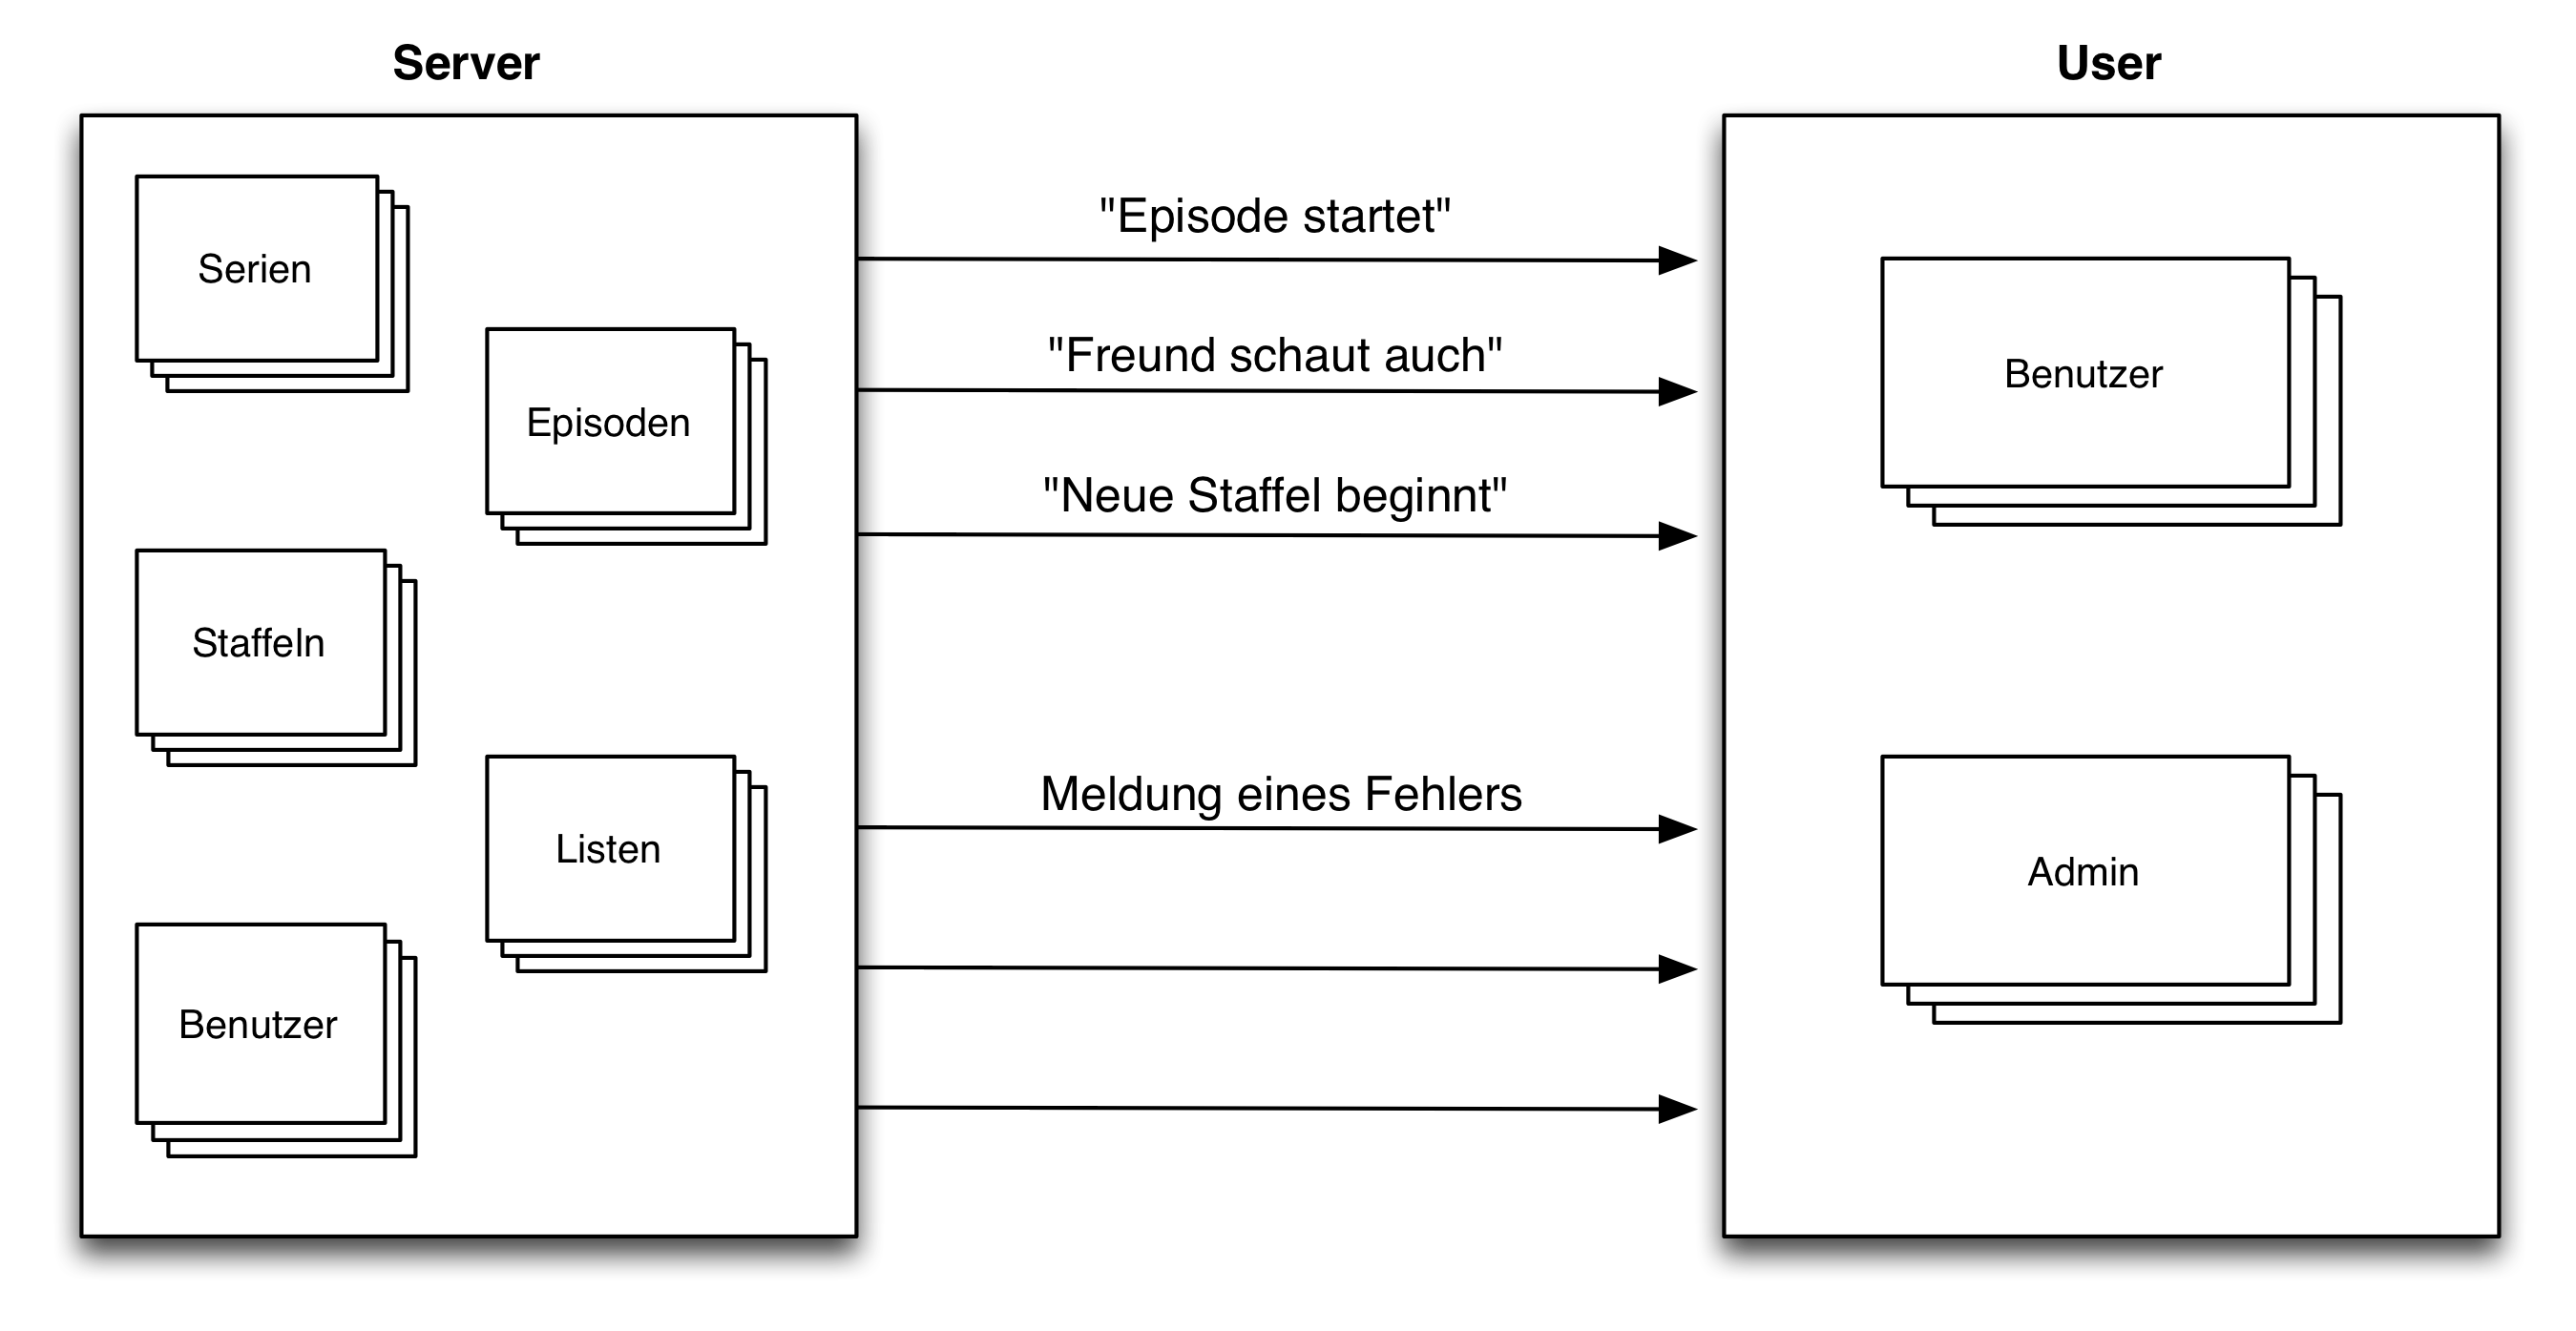
\includegraphics[width=1\textwidth]{images/kommunikationsablaeufeAsynchron.png}
\caption{Asynchrone Kommunikationsabläufe}
\label{kommunikationsablaeufeAsynchron}
\end{figure}



\begin{table}[H]
\caption{Ressourcen des Serientrackers}  % title name of the table\\

\centering % centering table
\begin{tabular}{l l l} % creating 10 columns
\hline\hline % inserting double-line
 \\ [-0.5ex]
 Ressource & URI & Methode
\\ [1ex]
\hline % inserts single-line
% Entering 1st row
Liste aller Serien & /series/ & GET, PUT \\[1ex]
Einzelne Serie & /series/\{id\} & GET, POST, DELETE\\[1ex]
Liste aller Staffeln & /seasons/ & GET, PUT \\[1ex]
Einzelne Staffel & /seasons/\{id\} & GET, POST, DELETE\\[1ex]
Liste aller Episoden & /episodes/ & GET, PUT \\[1ex]
Einzelne Episode & /episodes/\{id\} & GET, POST, DELETE\\[1ex]
Liste aller User & /users/ & GET, PUT \\[1ex]
Einzelne User & /users/\{id\} & GET, POST, DELETE\\[1ex]
Liste aller Listen & /lists/ & GET, PUT\\[1ex]
Liste eines Users & /lists/\{id\} & GET, POST, DELETE\\[1ex]
% [1ex] adds vertical space
\hline % inserts single-line
\end{tabular}
\label{tab:PPer}
\end{table}

\newpage

\section{Projektbezogenes XML Schema / Schemata}
Der erste Meilenstein befasst sich mit der Repräsentation von Daten in XML.

Damit bei der Verwendung der XML Dateien bei der späteren Verarbeitung mit JAXB keine Probleme auftreten,
ist es notwendig eine Validierung der Dateien durch Definition zugehöriger XML Schemas durchzuführen.
Vorteil bei der Verwendung eines Schemas ist, neben der Kontrolle auf Wohlgeformtheit und der Verwendung
definierter Datentypen und Strukturen, auch das festlegen von Restriktionen.

Hinsichtlich des zugrunde liegenden Konzeptes und den benötigten Informationen, gibt es viele Elemente
innerhalb der Dateien, die nur mit Strings realisiert werden können. Das Problem bei freier Definition
besteht darin, dass die Datensätze sehr fehleranfällig sind, wenn es um die Benutzung durch Menschen geht.
Rechtschreibfehler beim Namen des Landes, des Fernsehsenders oder des Genres, würden für den Leser bzw.
Interessenten der Anwendung noch kein Problem darstellen, da er vermutlich deuten könnte was gemeint ist.
Informationstechnisch ist es aber von Vorteil, die Datensätze möglichst konsistent und reichhaltig anzulegen.

Das System des Serientrackers beruht darauf, die Verwaltung von Serien anhand von Listen und Tags wie
Gesehen, Ungesehen zu ermöglichen. Wie bereits in der Besprechung der Umsetzung erwähnt, wird anhand
dieser Informationen auch die Asynchrone Datenübertragung realisiert.
Das Abonnieren von Informationen zu laufenden Serien des Genre Krimi, greift bei Benachrichtigung auf
Datensätze zu, die diesem Elementwert unter dieser eindeutigen Zeichenfolge zugeordnet sind. Formulierungsfehler
wie Krimie oder Crime, führen dementsprechend zu Komplikationen, weil sie die Reinheit der Informationssätze beschädigen.

Datentypen
Zu Beginn des ersten Meilensteins, steht die Analyse der vorhandenen Informationstypen.
Bei der Definition eines XML Schemas, sollte neben der enstprechenden Datensatzstruktur und Reihenfolge,
auch festgelegt werden, durche welche Datentyp die einzelnen Informationen repräsentiert werden sollen.

\newpage

\begin{figure}[H]
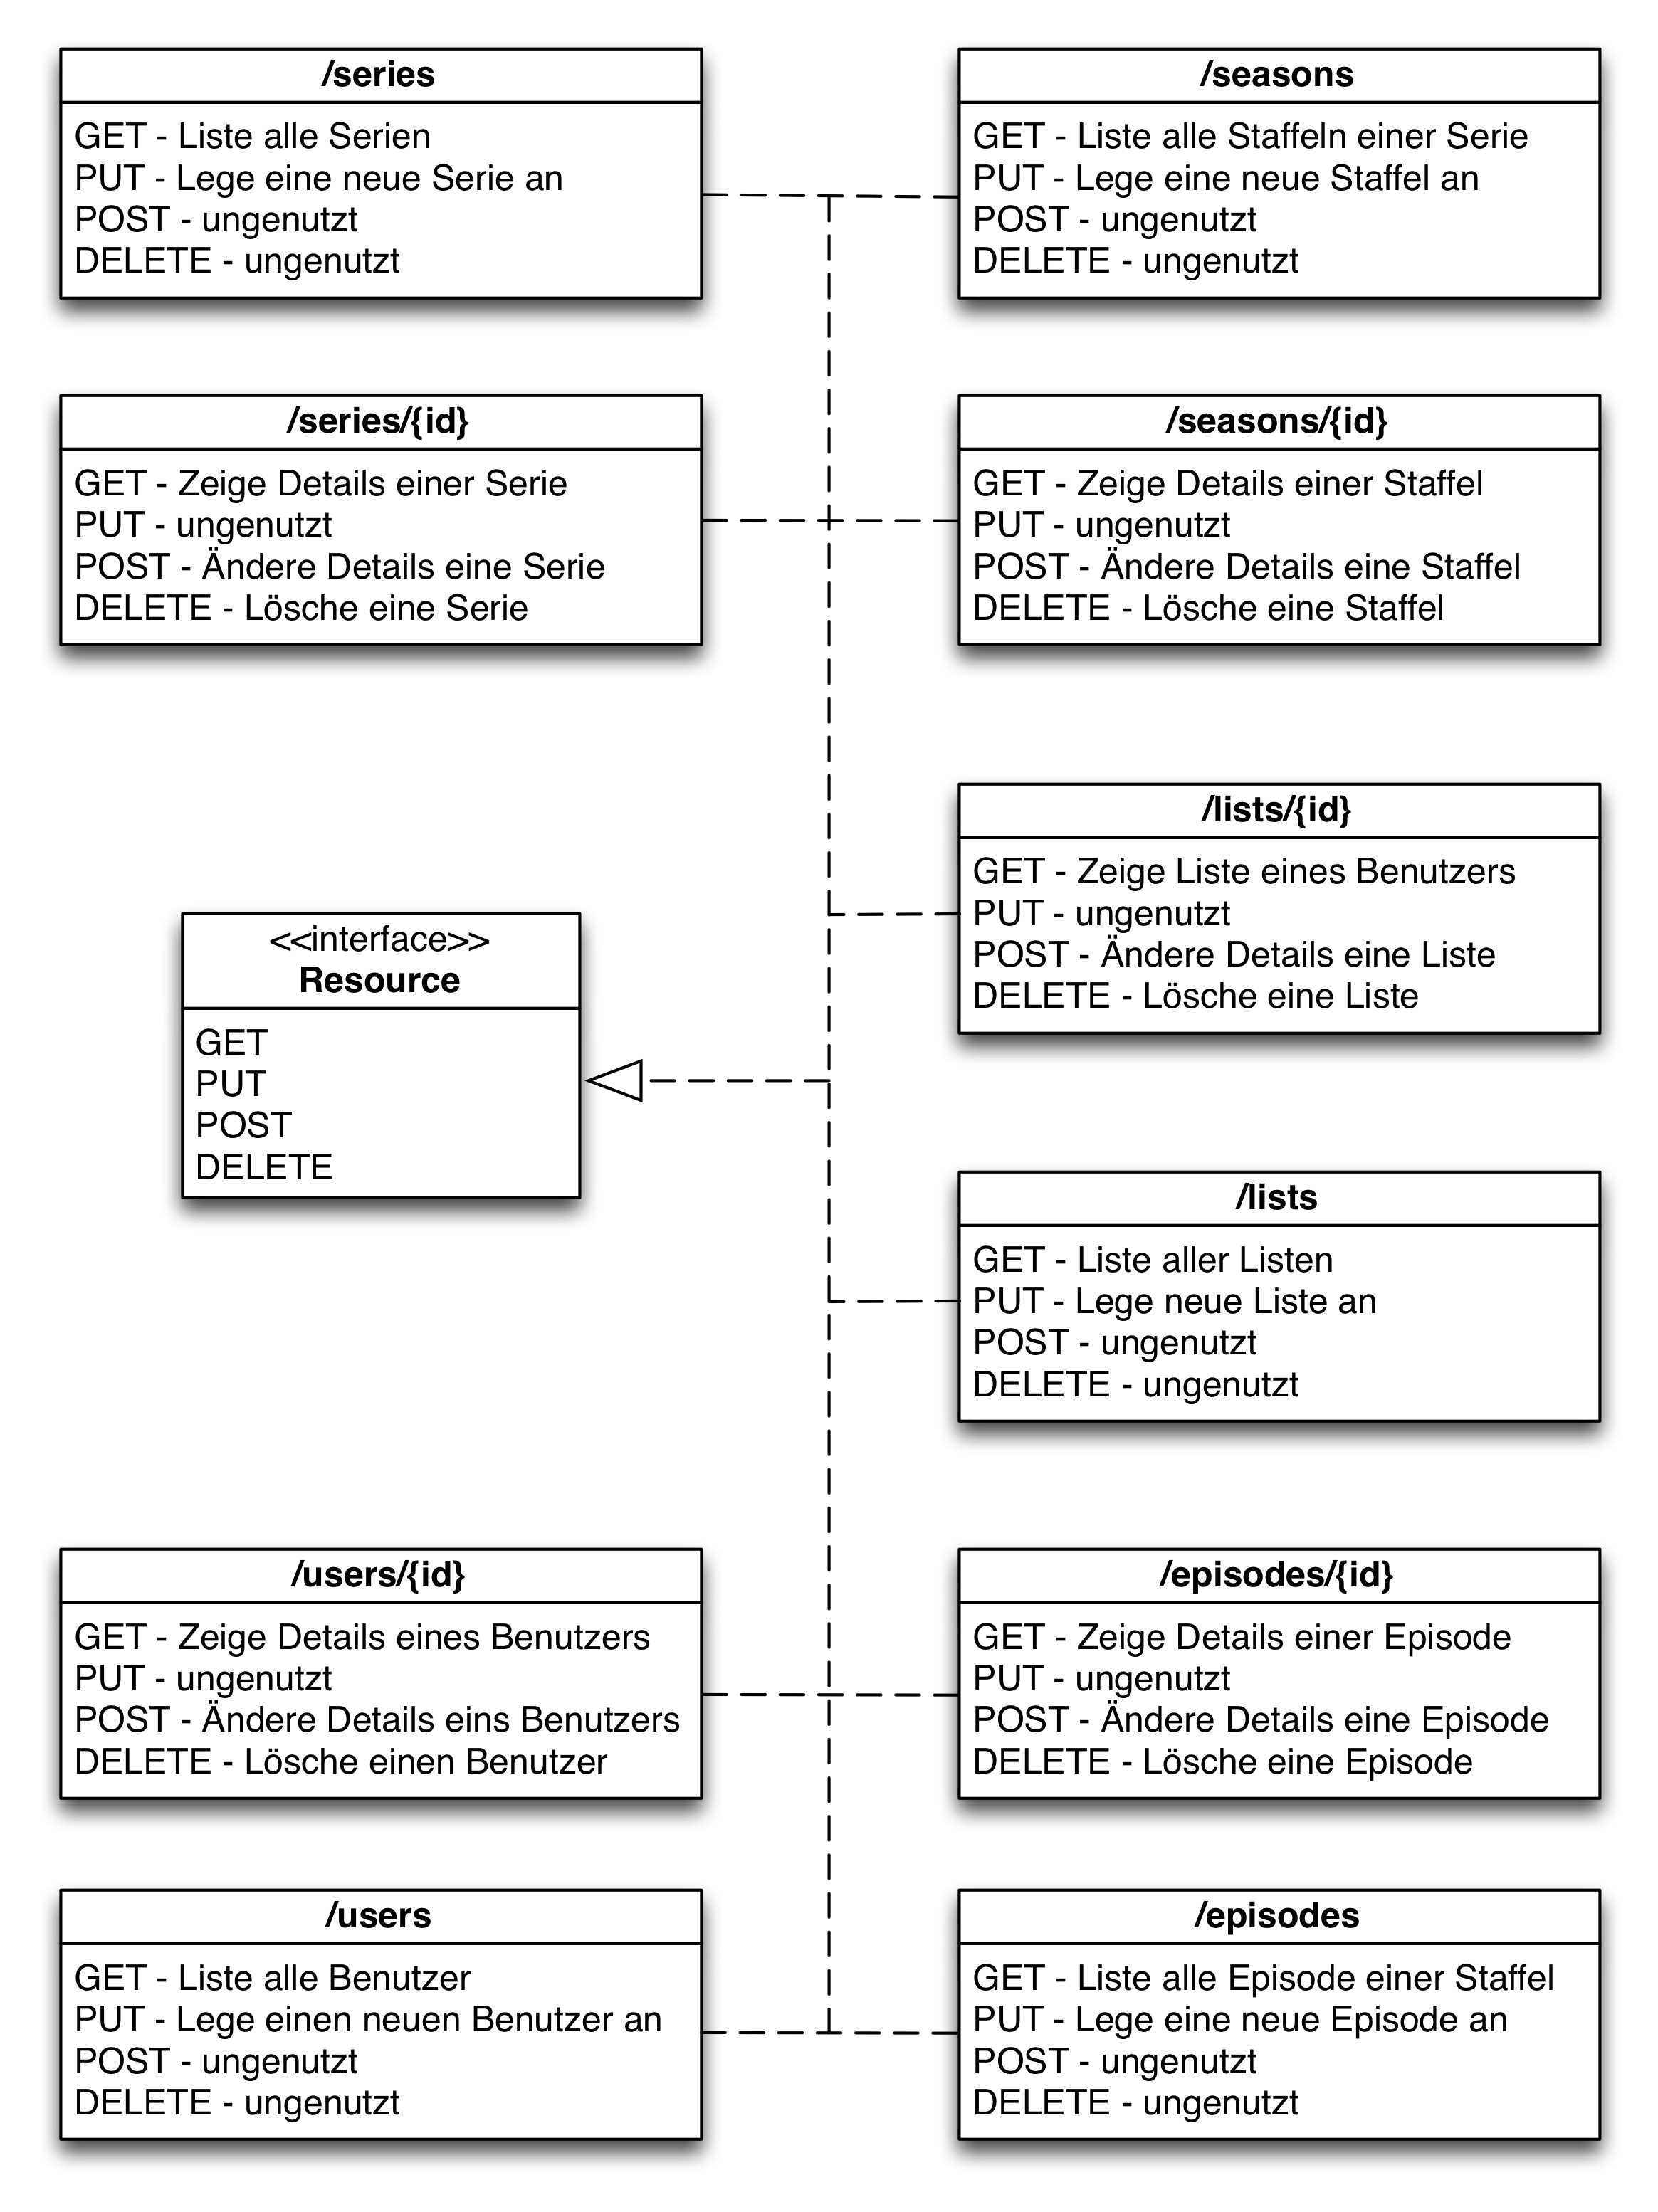
\includegraphics[width=1\textwidth]{images/bedeutunghttpmethoden.png}
\caption{Bedeutung der http Methoden}
\label{bedeutunghttpmethoden}
\end{figure}

\newpage



\listoffigures





\end{document}
